%*******************************************************************************
% Master TeX file for 7.5x9.25 books
% Copyright A K Peters, Ltd.
%
% This is the main TeX file that is to be compiled.  Rename the file as needed.
%*******************************************************************************
\documentclass{book}

%*******************************************************************************
% Layout
%*******************************************************************************
\usepackage[dvips,showcrop,letterpaper]{geometry}

\geometry{
layouthoffset=0.5in,
  layoutvoffset=0.875in,
  layoutwidth=7.5in,
  layoutheight=9.25in,
  width=27pc,
  height=45.5pc, % textheight + head + headsep = 45pc
  headsep=20pt,
  foot=26pt,
  inner=0.25in, % gutter margin
  top=0.75in, % head margin
  includehead
}

%*******************************************************************************
% Style file
%*******************************************************************************
\usepackage{akpbook}

%*******************************************************************************
% Packages
%*******************************************************************************
%---BEGIN AUTHOR EDIT---

%---END AUTHOR EDIT---

%*******************************************************************************
% Declarations
%   Any custom commands, aliases, or other declarations should be added below,
%   either inline or by including an external TeX file (e.g. \include{MyMacros})
%*******************************************************************************
%---BEGIN AUTHOR EDIT---

%---END AUTHOR EDIT---

%*******************************************************************************
% Figure folders
%   For most authors, figures will be .eps files.  These figures should be
%   contained in any number of subfolders below the root folder.  Use the
%   following syntax to point to those folders:
%
%   \graphicspath{ {folder1/} {folder2/} {folder2/subfolder1/} }
%
%   Figures can then be included in the document using:
%
%   \includegraphics[width=\textwidth](FigFileName.eps}
%
%   or similar command.
%*******************************************************************************
%\graphicspath{} % you may uncomment this line if needed

%*******************************************************************************
% Workspace
%
% Use \includeonly{chapter1, chapter2, chapter3} to limit the files tex'ed
%*******************************************************************************
%\includeonly{} % you may uncomment this line if needed

%*******************************************************************************
% Book
%*******************************************************************************
\makeindex % uncomment this line if you need to generate an index
\begin{document}

%*******************************************************************************
% Front Matter%
%   The table of contents follows which is generated by \tableofcontents.
%
%   For final production, the generated *.toc file must be renamed to toc.tex.
%   This file can be edited as needed like any other included tex file.  Make
%   sure that the \tableofcontents command remains commented-out for the final
%   version of the TOC.
%
%   Next is the preface file.  Edit the text in preface.tex.
%
%   Additional front matter sections can be added as needed such as lists of
%   symbols.
%*******************************************************************************
\frontmatter
 \pagestyle{empty}
 %*******************************************************************************
% Front Matter TeX file for books
% Copyright A K Peters, Ltd.
%*******************************************************************************
\vspace*{1in}

 \begin{flushright}
 \setlength{\baselineskip}{30pt}
 {\MTSMALL The WebGL Companion}
 \end{flushright}

\newpage

\phantom{Xx}

\newpage

%\vspace*{0.5in}

 \begin{flushright}
 \setlength{\baselineskip}{36pt}
 {{\MT The WebGL Companion}\\{\MTSUB }}

\vspace{1in}

 \setlength{\baselineskip}{22pt}
 {\MTA Philip Rideout}

\vfill

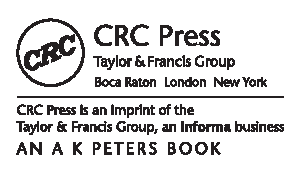
\includegraphics{AKPeters_TitlePageLogo.eps}

 \end{flushright}

\newpage

COPYRIGHT PAGE TO BE INSERTED

\newpage


\vspace*{1in}


\begin{flushright}
 \setlength{\baselineskip}{13.5pt}
{\MTD Dedicated to Allan Rideout.}
\end{flushright}

\newpage
\strut
 % title and copyright pages

 \pagestyle{fancy}
 \renewcommand{\chaptermark}[1]{\markboth{#1}{#1}}
 \renewcommand{\sectionmark}[1]{}

 \tableofcontents % uncomment this line if you need to generate a TOC
% \include{toc} % use and edit for final version
 %*******************************************************************************
% Preface TeX file for books
% Copyright A K Peters, Ltd.
%*******************************************************************************
\chapterstar{Preface}

%---BEGIN AUTHOR EDIT---
Lorem ipsum dolor sit amet, consectetuer adipiscing elit. Duis
sapien ligula, sollicitudin eget, pulvinar in, condimentum et,
leo. Nullam sagittis sem in massa. Donec tortor sem, pulvinar
quis, nonummy sit amet, ultricies a, justo. Proin sollicitudin
libero vel lorem. Aliquam erat volutpat. Etiam faucibus fringilla
dolor. Duis in orci. Pellentesque ultricies velit a lacus. Sed
cursus est. Praesent vitae erat. Ut est ante, consectetuer a,
laoreet feugiat, auctor non, erat. Nullam dui. Phasellus interdum
libero vel ligula. Cras pretium lorem id dolor. Nullam auctor,
leo at vulputate viverra, orci lorem nonummy lorem, nec bibendum
nunc tortor eu orci. Nam nec leo. Nunc dolor. Praesent in sapien
vitae diam lacinia feugiat. Sed nec lectus vel tortor ultrices
congue.

Fusce commodo orci id nunc. Pellentesque porttitor tincidunt
massa. Fusce blandit quam malesuada magna. Nunc tempus. Cras est
mi, mollis congue, egestas at, rutrum id, mi. Sed pede ante,
commodo convallis, blandit et, nonummy quis, nisl. Pellentesque
id dui sed lorem ultrices commodo. Nullam felis augue,
condimentum sit amet, fringilla rhoncus, vehicula id, tortor.
Donec erat diam, semper vel, vehicula vitae, ullamcorper in,
arcu. Sed sed lacus. Aenean ut massa. Quisque lacinia auctor
sapien. Morbi velit ligula, rhoncus eu, fringilla vel, tempor
vitae, nibh. Aliquam erat volutpat. Proin euismod libero at
mauris.

Maecenas leo leo, pretium a, tincidunt a, hendrerit a, velit. In
hac habitasse platea dictumst. Sed gravida. Praesent nunc. Morbi
pulvinar molestie erat. Maecenas congue rhoncus sem. Cras in
neque vitae orci tincidunt sagittis. Donec vehicula enim at leo.
Nullam et metus. Ut pede. Proin pretium massa. Nulla semper
egestas nisl. Maecenas sollicitudin. Vestibulum imperdiet, diam
eu varius imperdiet, velit mi lobortis augue, eget cursus ligula
lorem quis mauris. Mauris libero massa, ornare sed, ullamcorper
eget, fringilla non, elit. Curabitur tortor pede, iaculis ac,
volutpat sit amet, scelerisque in, arcu. Pellentesque ut lorem ac
leo vestibulum fringilla. Nullam neque ante, tempor a, suscipit
sit amet, scelerisque et, dolor.

Mauris in eros. Vivamus luctus. Suspendisse potenti. Sed et neque
et tortor pretium iaculis. Etiam malesuada iaculis pede. Aenean
congue lobortis lectus. Nulla nonummy, elit gravida tincidunt
pulvinar, odio tortor tempor sem, a facilisis odio diam non
ipsum. Donec rhoncus quam ut velit. Integer non mi eu justo
iaculis feugiat. Aliquam turpis. Aliquam lobortis blandit lectus.
Pellentesque habitant morbi tristique senectus et netus et
malesuada fames ac turpis egestas. Sed libero est, aliquam vel,
laoreet nec, dignissim ut, justo. Sed nec tellus. Cras a dui id
ipsum laoreet varius. Pellentesque eleifend arcu sit amet dui.

Vestibulum consectetuer convallis pede. Ut consectetuer lectus
vitae odio. Nunc volutpat pede non turpis. Suspendisse potenti.
Aenean suscipit tempor nunc. Sed sollicitudin rhoncus purus.
Donec at enim sed urna gravida dapibus. Curabitur eget lorem.
Vivamus interdum magna nec felis. Phasellus cursus semper lectus.
Donec mollis justo ac orci. Pellentesque habitant morbi tristique
senectus et netus et malesuada fames ac turpis egestas.
Pellentesque egestas leo suscipit ipsum.
%---END AUTHOR EDIT---

%---BEGIN AUTHOR EDIT---

%---END AUTHOR EDIT---

%*******************************************************************************
% Parts and chapters
%   \part{Part 1} where "Part 1" is the part title
%   \include{chapter1) where "chapter1" is the filename chapter1.tex
%*******************************************************************************
\mainmatter
 \renewcommand{\chaptermark}[1]{\markboth{\thechapter. #1}{}}
 \renewcommand{\sectionmark}[1]{\markright{\thesection. #1}}
%---BEGIN AUTHOR EDIT---
%*******************************************************************************
% Example chapter file for books
% Copyright A K Peters, Ltd.
%*******************************************************************************
\chapter{Example Chapter}%{John Doe}
 \label{ch1}

% if you want to include the author's name below the title, add the second argument to the \chapter opening as above and remove the %:


Lorem ipsum dolor sit amet, consectetuer adipiscing elit.
Maecenas et mauris. Vestibulum pretium posuere enim. Quisque
ornare vehicula diam. Etiam ullamcorper nibh et purus. Class
aptent taciti sociosqu ad litora torquent per conubia nostra, per
inceptos hymenaeos. Quisque diam neque, elementum eu, pharetra
vitae, mollis semper, wisi. Aliquam accumsan convallis tortor.
Quisque quis neque. Vestibulum pede wisi, tempus nec, molestie
in, sollicitudin in, quam. Pellentesque cursus nisl quis lorem\index{index entry1}.

\[
y = \frac{-b \pm \sqrt{b^2 - 4ac}}{2a}
\]

\texttt{Mauris id mi.} \textbf{Aliquam velit enim,} \emph{lacinia
quis,} gravida ac, iaculis ac, odio. Pellentesque vulputate porta
dolor. In auctor convallis lorem. Vestibulum a justo in tortor
sagittis aliquam. Cras tortor. Nullam enim tellus, viverra quis,
sagittis luctus, malesuada eget, nulla. Nullam ac diam. Donec
pellentesque porttitor risus. Maecenas magna elit, laoreet eget,
tincidunt nec, gravida sit amet, felis. Fusce quis dui. Nunc felis \cite{doe:2004,doe:1994,hunt:1975}.

\section{Level One Head}

Nam turpis dui, iaculis et, convallis sit amet, euismod at, urna.
Vivamus urna quam, eleifend nec, tristique eget, rhoncus in,
libero. Vestibulum ante ipsum primis in faucibus orci luctus et
ultrices posuere cubilia Curae; Aliquam sagittis nonummy wisi.
Cras in magna. Donec luctus ornare nunc. Vivamus porta gravida
sem. Duis augue. Pellentesque pede est, condimentum vel, ornare
et, vulputate quis, quam. Cras risus sapien, ultricies sed,
lacinia ut, sodales sed, nunc. Sed consequat purus ac justo. In
hac habitasse platea dictumst. Vivamus convallis, ipsum et
tincidunt feugiat, quam arcu venenatis ligula, id cursus mauris
mi quis magna. Duis sed elit at nisl sollicitudin molestie. Nam
lacinia.

Duis turpis nunc, facilisis id, varius in, faucibus eu, justo.
Praesent egestas sem vel leo mattis rutrum. Etiam in massa nec
elit pharetra varius. Duis metus. Nunc tincidunt purus at velit.
Aenean fermentum est a eros. Nulla massa. Nulla tellus magna,
sagittis et, gravida at, euismod eget, ligula. Nunc eu risus et
wisi elementum scelerisque. Nulla a eros. Etiam ornare aliquet
enim. Nulla facilisi. Sed rutrum magna sit amet libero. Nunc sed
elit.

Aliquam feugiat. Vivamus posuere, leo ut sagittis porttitor,
augue nibh commodo sapien, eget fringilla arcu arcu eget wisi.
Duis a orci. Maecenas ornare, dolor id vehicula auctor, felis
metus volutpat nunc, id varius eros enim vel quam. Suspendisse
sapien. Aenean et elit ac neque nonummy laoreet. Cras sit amet
orci. Donec ac tortor. Cum sociis natoque penatibus et magnis dis
parturient montes, nascetur ridiculus mus. Vestibulum pharetra.
Vivamus vitae risus. In hac habitasse platea dictumst. Nullam
elementum turpis eget magna. Vestibulum cursus, eros nec porta
rutrum, augue est suscipit nisl, non pellentesque lacus dui eu
nibh.

\subsection{Level Two Head}

In hac habitasse platea dictumst. Aliquam erat volutpat. In
aliquet ligula rhoncus erat. Vivamus id velit ac ligula malesuada
dapibus. Cras ac justo ac elit feugiat tincidunt. Vivamus diam
nulla, ultricies sed, condimentum sit amet, facilisis a, massa.
Vestibulum feugiat vehicula nulla. Suspendisse potenti.
Pellentesque purus mi, fringilla ut, volutpat et, semper et,
felis. Donec quis tellus.

Mauris porta est. Vivamus justo mi, venenatis eget, mollis sed,
blandit posuere, dui. Cum sociis natoque penatibus et magnis dis
parturient montes, nascetur ridiculus mus. Nam rhoncus. Aliquam
lobortis tempor neque. Lorem ipsum dolor sit amet, consectetuer
adipiscing elit. Quisque feugiat molestie lectus. In interdum
sodales est. Aliquam erat volutpat. Integer feugiat. Suspendisse
elit. Aliquam porta, orci sit amet sollicitudin adipiscing,
sapien est congue quam, vitae egestas sem felis vel augue. Donec
vitae lacus et dui mollis fermentum. Suspendisse potenti. Donec
faucibus, est id porta cursus, quam purus malesuada dolor,
bibendum aliquet nunc velit sit amet magna.

\subsubsection{Level Three Head}

Integer odio risus, adipiscing sed, aliquam vitae, pulvinar sit
amet, dolor. Morbi eget purus. Curabitur sollicitudin libero a
leo. Duis id arcu. Donec est odio, feugiat at, sagittis ut,
euismod eget, elit. Integer odio. Etiam consectetuer suscipit
nunc. Sed tincidunt. Pellentesque lobortis adipiscing sapien.
Proin mauris turpis, nonummy eget, fermentum ac, aliquet et,
erat. Vivamus quis augue. Aliquam nec mauris a tellus
consectetuer lacinia. Morbi diam.

\subsubsection{Level Three Head}

Pellentesque habitant morbi tristique senectus et netus et
malesuada fames ac turpis egestas. Suspendisse pede. Phasellus
bibendum scelerisque orci. Nulla scelerisque, magna a eleifend
rutrum, magna dui ornare diam, eget rhoncus augue wisi at leo.
Sed et nibh. Vestibulum condimentum sagittis libero. Vestibulum
vehicula varius nibh. Donec non nisl. Suspendisse ac sem quis
lorem tincidunt commodo. Nunc aliquet, metus nec blandit feugiat,
pede neque tincidunt ante, elementum lobortis metus turpis quis
justo. Quisque quis urna. Aenean quis enim suscipit metus
malesuada ultricies. Donec scelerisque sollicitudin magna. Cras
at quam a ipsum faucibus nonummy. Sed venenatis nulla sit amet
arcu. Quisque quam urna, lacinia quis, luctus nec, pharetra vel,
lacus.

\subsubsection{Level Three Head}

Duis malesuada, lectus sed bibendum laoreet, odio ipsum egestas
velit, eget scelerisque enim risus nec nulla. Mauris interdum
tortor in nulla. Aliquam vitae eros sed eros cursus dictum. Etiam
metus. In bibendum tincidunt neque. Morbi nonummy rhoncus sapien.
Fusce vitae dolor et leo pretium mattis. Praesent dictum
pellentesque nibh. Curabitur faucibus. Donec imperdiet vulputate
elit. Nullam nec leo et elit laoreet iaculis. Nulla est elit,
adipiscing id, aliquam in, accumsan vel, sapien. Proin
pellentesque posuere elit. Nulla facilisi\index{index entry2}.

\subsection{Level Two Head}

In hac habitasse platea dictumst. Aliquam erat volutpat. In
aliquet ligula rhoncus erat. Vivamus id velit ac ligula malesuada
dapibus. Cras ac justo ac elit feugiat tincidunt. Vivamus diam
nulla, ultricies sed, condimentum sit amet, facilisis a, massa.
Vestibulum feugiat vehicula nulla. Suspendisse potenti.
Pellentesque purus mi, fringilla ut, volutpat et, semper et,
felis. Donec quis tellus.

Mauris porta est. Vivamus justo mi, venenatis eget, mollis sed,
blandit posuere, dui. Cum sociis natoque penatibus et magnis dis
parturient montes, nascetur ridiculus mus. Nam rhoncus. Aliquam
lobortis tempor neque. Lorem ipsum dolor sit amet, consectetuer
adipiscing elit. Quisque feugiat molestie lectus. In interdum
sodales est. Aliquam erat volutpat. Integer feugiat. Suspendisse
elit. Aliquam porta, orci sit amet sollicitudin adipiscing,
sapien est congue quam, vitae egestas sem felis vel augue. Donec
vitae lacus et dui mollis fermentum. Suspendisse potenti. Donec
faucibus, est id porta cursus, quam purus malesuada dolor,
bibendum aliquet nunc velit sit amet magna.

\subsubsection{Level Three Head}

Integer odio risus, adipiscing sed, aliquam vitae, pulvinar sit
amet, dolor. Morbi eget purus. Curabitur sollicitudin libero a
leo. Duis id arcu. Donec est odio, feugiat at, sagittis ut,
euismod eget, elit. Integer odio. Etiam consectetuer suscipit
nunc. Sed tincidunt. Pellentesque lobortis adipiscing sapien.
Proin mauris turpis, nonummy eget, fermentum ac, aliquet et,
erat. Vivamus quis augue. Aliquam nec mauris a tellus
consectetuer lacinia. Morbi diam.

\subsubsection{Level Three Head}

Pellentesque habitant morbi tristique senectus et netus et
malesuada fames ac turpis egestas. Suspendisse pede. Phasellus
bibendum scelerisque orci. Nulla scelerisque, magna a eleifend
rutrum, magna dui ornare diam, eget rhoncus augue wisi at leo.
Sed et nibh. Vestibulum condimentum sagittis libero. Vestibulum
vehicula varius nibh. Donec non nisl. Suspendisse ac sem quis
lorem tincidunt commodo. Nunc aliquet, metus nec blandit feugiat,
pede neque tincidunt ante, elementum lobortis metus turpis quis
justo. Quisque quis urna. Aenean quis enim suscipit metus
malesuada ultricies. Donec scelerisque sollicitudin magna. Cras
at quam a ipsum faucibus nonummy. Sed venenatis nulla sit amet
arcu. Quisque quam urna, lacinia quis, luctus nec, pharetra vel,
lacus.

\subsubsection{Level Three Head}

Duis malesuada, lectus sed bibendum laoreet, odio ipsum egestas
velit, eget scelerisque enim risus nec nulla. Mauris interdum
tortor in nulla. Aliquam vitae eros sed eros cursus dictum. Etiam
metus. In bibendum tincidunt neque. Morbi nonummy rhoncus sapien.
Fusce vitae dolor et leo pretium mattis. Praesent dictum
pellentesque nibh. Curabitur faucibus. Donec imperdiet vulputate
elit. Nullam nec leo et elit laoreet iaculis. Nulla est elit,
adipiscing id, aliquam in, accumsan vel, sapien. Proin
pellentesque posuere elit. Nulla facilisi.

%---END AUTHOR EDIT---

%*******************************************************************************
% Back Matter
%   Back matter begins with the bibliography.  We strongly recommend using a
%   .bib file.  You are welcome to use another bibliography style instead of our
%   in-house style.  For final production, the generated file can be renamed to
%   bibliography.tex. This file can be edited as needed, usually to fix breaks.
%
%   The index follows.  The index is generated using \makeindex (see above).
%   Use \printindex to display the index.
%
%   For final production, the generated file can be renamed to index.tex.
%   This file can be edited as needed.  Make sure that the \makeindex and
%   \printindex commands remain commented-out for the final version of the
%   index.
%*******************************************************************************
\backmatter
 \renewcommand{\chaptermark}[1]{\markboth{#1}{#1}}

\small

\bibliographystyle{akpbib}
\bibliography{}
%\include{bibliography} % use and edit for final version



\raggedright  % fixes index problem
\printindex % uncomment to display the index during authoring
%\include{index} % use and edit for final version


% any unnumbered pages go here, typically a color insert.
 \pagestyle{plain}
 \fancyhf{}
\end{document}
